\chapter{Hardware-alvo}

%source: http://www.zedboard.org/product/zedboard
% http://www.zedboard.org/sites/default/files/documentations/ZedBoard_HW_UG_v2_2.pdf
Zedboard é uma plataforma de desenvolvimento que suporta uma grande variedade de aplicações, visto que ela possui uma boa gama de interfaces e funções para habilitar isto. É dedicada à prototipação e \emph{proof-of-concept}. Em seu interior ela possui um Xilinx Zynq 7000 (Z-7020), que é a arquitetura alvo deste porte. A figura \ref{fig:zedboard} mostra como é a placa fisicamente. Zynq 7020 possui um processador \emph{dual core} Cortex A9, cada core possui sua própria MMU e memória cache L1 (instruções e dados) privada.

O ZYNQ-7000 SOC XC7Z020-CLG484-1 conta com o processador Dual ARM Cortex-A9 MPCore. O Zynq possui 4 graduações de velocidade de \emph{clock}, a comercial (graduação -1), industrial (graduação -1 a -2), estendida (-2 a -3) e expandida (-1), sendo a graduação -1 a menor velocidade, e a -3 a maior \cite{product_table}.

De acordo com a especificação da Zedboard \cite{zedboard}, o \emph{clock} máximo do processador é de 667MHZ, portanto, tendo como referência a tabela de dados do Zynq-7000 \cite[p.~13]{data_sheet}, chegamos à conclusão que a graduação de velocidade do Zynq usado na Zedboard é de -1 (comercial), esta informação se tornará útil mais à frente.

Há disponível 512MB de RAM DDR3, e um SD card de 4GB. A Zedboard suporta conexão com JTAG, saída serial (USB UART) e conexão com a internet \cite{xilinx}.

A família Zynq 7000 disponibiliza para o desenvolvedor FPGAs, tornando esta plataforma mais configurável e flexível \cite[p.~26]{ug585}. A PS dessa família é a mesma para cada dispositivo onde ela se encontra, entretanto a PL e recursos de entrada e saída variam entre diferentes dispositivos. 


\begin{figure}[ht!]
	\label{fig:zed}
    \centering
    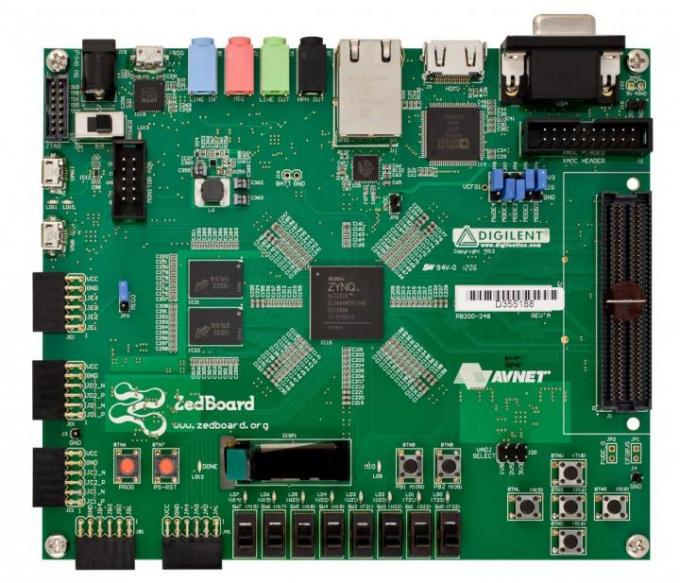
\includegraphics[width=8cm]{figuras/zedboard}
	\label{fig:zedboard}
    \caption{Zedboard visto de cima.}
\end{figure}

%layout de memoria
\section{OCM} O \emph{On-chip Memory} é uma pequena memória de 256KB de RAM que fica próxima ao processador, e portanto tem um acesso mais rápido. O OCM pode ser mapeado nos primeiros 256KB do espaço de endereçamento, ou nos últimos 256KB do espaço de endereçamento \cite{ug585}.


\section{Modos de Operação}
\label{sec:operating_modes}
A arquitetura ARMv7 conta com 9 modos de operação (7 por padrão, mais 2 com extensões habilidadas), sendo que o único modo não privilegiado é o modo de usuário, os demais modos padrão possuem o mesmo privilégio dentro do sistema\footnote{O modo hipervisor possui certas funções que os demais modos não oferecem, mas no que diz respeito à acesso a memória e execução de instruções, ainda é o mesmo nível de privilégio.}. A principal diferença entre um modo e outro é que cada modo conta com um certo subconjunto privado de registradores banqueados, visiveis somente no modo em vigência, como ilustra a figura \ref{fig:banked}. A tabela \ref{tab:processormode} ilustra quais são os modos de operação disponíveis \cite[p.~1139]{armarm}.
O campo ``Codificação'' é usado no registrador CPSR para se verificar ou modificar o modo de operação vigente.

\begin{table}[ht]
\centering
\begin{tabular}{ccc}
\hline\hline                        %inserts double horizontal lines
Modo do processador  & Codificação & Implementado?\\ [0.5ex]
%heading
\hline                  % inserts single horizontal line
User & 10000 & Sempre \\
FIQ & 10001 & Sempre \\
IRQ & 10010 & Sempre \\
Supervisor & 10011 & Sempre\\
Monitor & 10110 & Com extensões de segurança.\\
Abort & 10111 & Sempre\\
Hyp & 11010 & Com extensões de virtualização.\\
Undefined & 11011 & Sempre\\
System & 11111 & Sempre\\[1ex]
\hline %inserts single line
\end{tabular}
\caption{Modos do processador. Codificação corresponde aos bits CPSR[4:0].}
\label{tab:processormode}
\end{table}

\textbf{Modo Usuário:} Modo não-privilegiado de execução. Neste modo somente é possível de se fazer acesso não privilegiado aos recursos do hardware (não podendo acessar as áreas protegidas). Não é possível mudar para outro modo de operação quando neste, a não ser por eventos externos como interrupções.

\textbf{Modo Sistema:} Modo privilegiado de execução. Este modo usa os mesmos registradores que o modo usuário e nenhuma exceção leva a este modo. Somente é possível de entrar nesse modo alterando os bits do registrador de status do sistema (CPSR); é necessário já estar em algum modo privilegiado para tal operação.

\textbf{Modo Supervisor:} É o modo padrão para no qual processador entra quando uma exceção do tipo \emph{Supervisor Call} é recebida.
Para gerar um \emph{Supervisor Call}, usa-se a instrução \verb+svc+. O processador entra neste modo ao se resetar.

\textbf{Modo Abort:} Modo que o processador entra quando recebe uma interrupção do tipo \emph{prefetch abort} ou \emph{data abort}.

\textbf{Modo Indefinido:} Modo que o processador entra quando se tenta executar uma instrução não definida ou mal formada.

\textbf{Modo FIQ:} Modo que o processador entra quando recebe uma interrupção FIQ.

\textbf{Modo IRQ:} Modo que o processador entra quando recebe uma interrupção IRQ.

\textbf{Modo Hipervisor:} Este modo possui alguns privilégios a mais que os demais modos, mas somente existe quando as extensões de virtualização estão ativas (fora do escopo deste trabalho).

\textbf{Modo Monitor:} Modo que o processador entra quando recebe uma interrupção \emph{Secure Monitor Call}, \verb+SMC+. Este modo está fora do escopo do trabalho.


\begin{figure}[ht!]
	\centerline{
    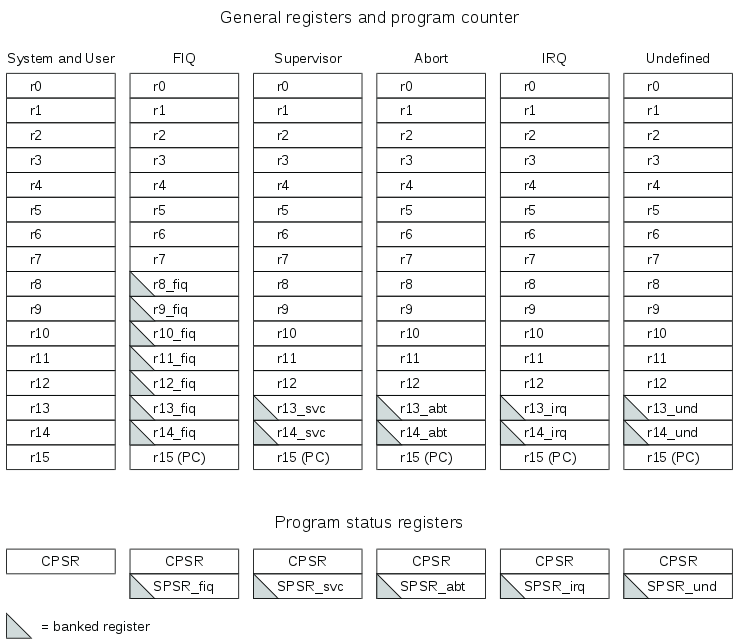
\includegraphics[width=12cm]{figuras/banked_registers}
	}
	\caption{Registradores banqueados (os modos especiais \emph{hypervisor} e \emph{monitor} não estão contemplados).}
	\label{fig:banked}
\end{figure}



\section{GIC}
O GIC (\emph{Generic Interrupt Controller}) é um componente que centraliza e administra todas as interrupções do sistema, ativando, desativando, mascarando e priorizando as fontes de interrupção.


\subsection{Tipos de Interrupção} %ug585 p. 192
\label{sec:interrupt}
\textbf{Interrupção Gerada por Software: }
Cada CPU pode se interromper, interromper outra CPU, ou ambas CPUs usando SGIs (\emph{Software Generated Interrupts}). Existem 16 interrupções geradas por software, que podem ser geradas escrevendo o número da interrupção ([0-15]), junto com o número da CPU alvo no registrador ICDSGIR. Esta escrita ocorre dentro do barramento privado da própria CPU. Cada CPU possui seu próprio conjunto privado de registradores de SGIs para gerarem uma (ou mais) das 16 SGIs possíveis \cite[p.~216]{ug585.1.7}. É possível limpar uma interrupção lendo o registrador ICCIAR (\emph{Interrupt Acknowledge}) ou escrevendo 1 nos bits correspondentes do registrador ICDICPR (\emph{Interrupt Clear-Pending}).
\\\\
\textbf{Interrupções de Periféricos Privados da CPU: }
\\\\
\textbf{Interrupções de Periféricos Compartilhados: }
Existem cerca de 60 interrupções de diversos modulos que podem ser roteadas para um ou ambos processadores, ou para a lógica programável. O GIC é responsável por administrar estas interrupções. Além das interrupções IRQ, há também interrupções do tipo FIQ e geradas por software.

\textbf{FIQ \emph{Fast Interrupt}:} O modo FIQ possui um número maior de registradores banqueados que os demais modos (R8 até R13, além do SP, LR e SPSR), fazendo com que não seja necessário fazer troca de contexto. FIQs também tem mais alta prioridade que qualquer IRQ, pontanto este tipo de interrupção é apropriado para aplicações de tempo real de usuário único. Se multiplas aplicações tempo real usarem FIQ, pode haver conflitos de interesse que podem fazer um processo perder um \emph{deadline} \cite[p.~66]{armarm}.

\textbf{Interrupção de Software: } Existe uma instrução no assembly do ARMv7 que permite que seja feita uma interrupção de software (\verb+swi+). Esta instrução pode ser acompanhada de um número de 8 bits. Esta interrupção leva ao modo supervisor.

%ARM ARM p. 66.

A Zedboard possui também as seguintes exceções\footnote{Em conceitos básicos está colocada a diferença entre interrupções e exceções}:

\textbf{Instrução não definida (\emph{Undefined Instruction}):} 
Há duas situações que geram esta interrupção: Quando se executa instruções de coprocessador que não são reconhecidas por este, ou quando se executa instruções que não possuem significado para o processador \cite[p.~36]{armarm}. Normalmente este tipo de interrupção acontecerá quando o processador estiver lendo e tentando executar lixo de memória.


\textbf{\emph{Prefetch Abort: }} Interrupção que leva ao modo \emph{Abort}. Este tipo de interrupção é sinalizado pelo sistema de memória (MMU). Através da MMU, é possível de se marcar certas regiões de memória como não executáveis; isto é importante de se fazer em regiões de memória que possuem dados sensíveis, de modo que quando o processador tentar ler aquela área para executar num futuro próximo, a MMU envia um sinal invalidando aquilo que foi lido. Quando o processador tenta executar uma instrução que tenha sido anteriormente invalidada, uma interrupção do tipo \emph{prefetch} ocorre \cite[p.~58]{armarm}. Note que é possível do processador ler aquela região para executar em seguida, mas ainda não gerar esta interrupção; isto ocorre quando o fluxo é desviado antes da tentativa de executar aquela instrução (por um \emph{branch} por exemplo).

\textbf{\emph{Data Abort:}} Assim como a \emph{prefetch abort}, esta interrupção também leva ao modo \emph{Abort} (e somente estas duas interrupções). Este tipo de interrupção pode acontecer quando uma instrução tenta acessar uma região de memória que o modo atual de execução não tenha permissão para acessar. Acesso a regiões de memória virtual não mapeadas pela MMU também geram esta interrupção.


%Source: http://infocenter.arm.com/help/index.jsp?topic=/com.arm.doc.dui0068b/BABFCEEG.html


\section{\emph{Timers}}
Cada um dos \emph{cores} possui um \emph{timer} privado de 32 bits e ambos \emph{cores} compartilham um \emph{timer} global de 64 bits. Estes \emph{timers} trabalham numa frequência sempre igual à metade da frequência da CPU.
No nível de sistema (\emph{system-level (PS)}), há dois grupos independentes de \emph{timers}, cada grupo com 3 \emph{timers}.


\section{\emph{Clocks}}

O \emph{clock} principal do sistema, chamado aqui de PS\_CLK (\emph{Processing System Clock}), é responsável por alimentar as 3 PLLs\footnote{\emph{Phase-Locked Loop}. É um sistema de controle que gera uma saída cuja fase é relacionada à fase do sinal de entrada. Pode ser usada para estabilizar um sinal e também multiplica-lo.} do sistema, sendo cada uma dessas PLLs responsável por uma parte diferente do sistema \cite[p.~622]{ug585}. O PS\_CLK é um \emph{clock} de baixa frequência, ficando entre 30 a 60 MHz (PS\_CLK é igual a 33.33 MHz no caso da Zedboard \cite[p.~19]{zed_manual}), sendo este multiplicado por cada uma das 3 PLLs para que o sistema funcione com velocidades maiores\footnote{Este clock pode ser multiplicado por um número de 1 a 127, e é multiplicado por 26 por padrão.}. As 3 PLLs são:

\begin{itemize}
	\item \textbf{I/O PLL:} Responsável por produzir o sinal de \emph{clock} para os dispositivos de entrada e saída.
	\item \textbf{DDR PLL:} Responsável por produzir o sinal de \emph{clock} para as memórias da plataforma.
	\item \textbf{ARM PLL:} Responsável por produzir o sinal de \emph{clock} do restante do sistema, incluindo os processadores.
\end{itemize}

A FPGA da Zedboard possui um \emph{clock} próprio e exclusivo. A figura \ref{fig:clocks} ilustra como estão dispostos estes \emph{clocks}.

\begin{figure}[ht!]
	\centerline{
    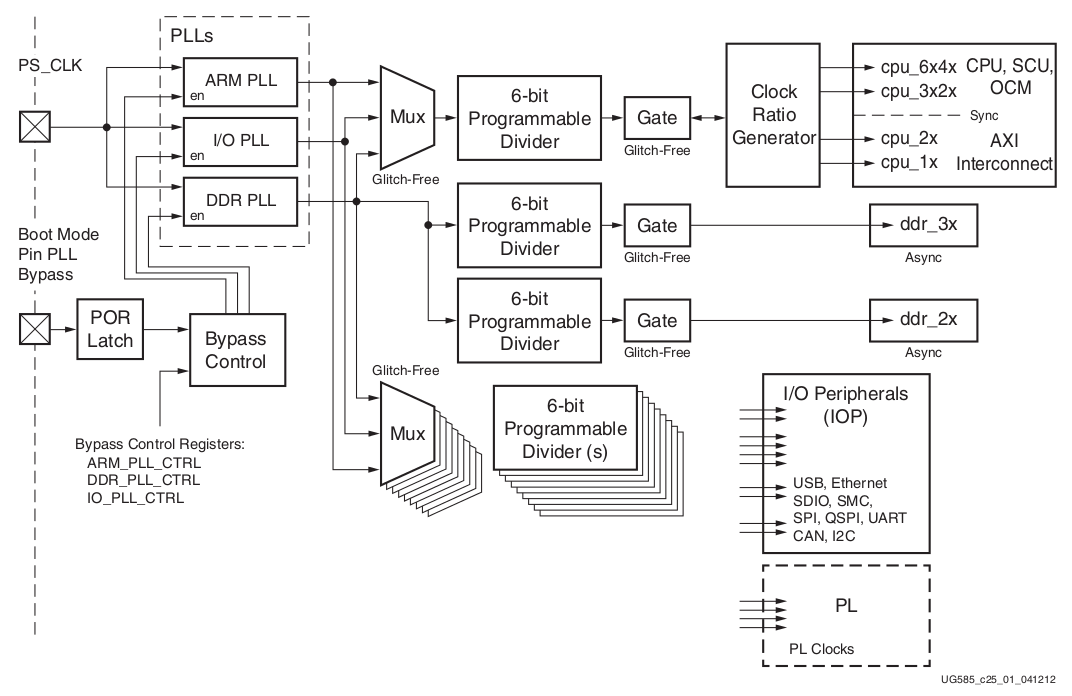
\includegraphics[width=13cm]{figuras/clocks}
	}
    \caption{Diagrama de blocos dos \emph{clocks} disponíveis no Zynq. Note os \emph{clocks} da tabela \ref{tab:clocks} no canto superior direito da imagem.}
	\label{fig:clocks}
\end{figure}

A Zedboard pode operar em dois modos (ou velocidades), denominados pela pela razão 6:3:2:1 e 4:2:2:1, abreviados como 6:2:1 e 4:2:1. Para alternar entre estes dois modos de velocidade, basta escrever 1 ou 0 no registrador CLK\_621\_TRUE. Estes números indicam quantas vezes cada \emph{clock} multiplica o \emph{clock} de base CPU\_1x, sendo este CPU\_1x um \emph{clock} derivado da ARM PLL, dividido por algum fator (configurável).

Há 4 \emph{clocks} independentes, chamados de CPU\_6x4x, CPU\_3x2x, CPU\_2x e CPU\_1x. Esta nomenclatura dos \emph{clocks} indica o fator pelo qual o CPU\_1x é multiplicado em cada modo.
O primeiro número do nome indica o fator multiplicativo daquele \emph{clock} no modo 6:2:1, e o segundo número indica o fator multiplicativo no modo 4:2:1.
Por exemplo, no modo \textbf{6}:2:1, o CPU\_\textbf{6x}4x multiplica o CPU\_1x 6 vezes, e no modo \textbf{4}:2:1, o CPU\_6x\textbf{4x} multiplica o CPU\_1x 4 vezes. A tabela \ref{tab:clocks} ilustra a velocidade de cada \emph{clock} em cada um dos dois modos.

\begin{table}[ht]
	\centering
	\begin{tabular}{ccc}
		\hline\hline
		\emph{Clock} & \emph{Clock Ratio Mode} & Máxima frequência da CPU\\[0.5ex]
		\hline
		CPU\_6x4x & \multirow{4}{*}{6:3:2:1} & 667 MHZ\\
		CPU\_3x2x &                          & 333 MHZ\\
		CPU\_2x   &                          & 222 MHZ\\
		CPU\_1x   &                          & 111 MHZ\\
		\hline
		CPU\_6x4x & \multirow{4}{*}{4:2:2:1} & 533 MHZ\\
		CPU\_3x2x &                          & 267 MHZ\\
		CPU\_2x   &                          & 267 MHZ\\
		CPU\_1x   &                          & 133 MHZ\\[1ex]
		\hline
	\end{tabular}
	\caption{Máximas frequências possíveis para cada configuração de \emph{clock}. Para uma lista mais completa (com as diferentes graduações de \emph{clock}), veja \cite[p.~13]{data_sheet}.}
	\label{tab:clocks}
\end{table}



%Faltou seção para a MMU e UART... Está bem explicado do capítulo do porte,
%mas seria coerente colocar alguma coisa aqui também...



